\documentclass[preprint]{elsarticle}
%\usepackage[english]{babel}
\usepackage[english]{babel}


\usepackage{subcaption}
\usepackage{graphicx}
\usepackage{hyperref}
\usepackage[table,xcdraw]{xcolor}
\usepackage[utf8]{inputenc}
\usepackage{setspace}
\usepackage{amssymb}
\usepackage{listings}
\usepackage{url}
\usepackage{pythonhighlight}

\usepackage{xcolor}
\usepackage[T1]{fontenc}
\newcommand\myworries[1]{\textcolor{red}{#1}}

\usepackage{enumitem}
\usepackage{float}
\usepackage{hyperref}
\usepackage{tikz}
\usepackage{multirow}
\usepackage{todonotes}
\usepackage{amsmath, amssymb}
\usepackage{placeins}
\usepackage{pdflscape}
\usepackage{amsthm}

\usepackage{graphicx}  
\usepackage{array}
\usepackage{booktabs} 
\usepackage{pifont}



\begin{document}
\begin{frontmatter}


\title{Generating Deepfakes with Stable Diffusion,\\ ControlNet and LoRA}





\author[perugia]{Stefano Bistarelli}
\ead{stefano.bistarelli@unipg.it}
\author[perugia]{Francesco Santini\corref{cor1}}
\ead{francesco.santini@unipg.it}
\author[perugia]{Edoardo Tavassi}
\ead{edoardo.tavassi@unipg.it}


\address[perugia]{Dipartimento di Matematica e  Informatica, University of Perugia, Italy}
\cortext[cor1]{Corresponding author}




\begin{abstract} 
???
\end{abstract}

\begin{keyword}
abstract argumentation, weighted attacks, sceptical semantics, unicity, well-founded frameworks.
\end{keyword}
\end{frontmatter}

%\linenumbers


\section{Introduction}


Deepfakes have become a popular subject of discussion in recent years. 
Advances in machine learning and artificial intelligence have made it possible to 
create highly realistic digital media that can deceive even the most discerning eye. 
However, creating convincing Deepfakes that are both stable and high-quality has proven 
to be challenging, requiring advanced techniques and algorithms. 
In this thesis, we will explore a novel approach to Deepfakes creation using 
Stable Diffusion, ControlNet, and LoRA, three recently proposed techniques that 
have shown promising results in various image synthesis tasks. 
In this thesis, we will comprehensively analyze all the technology needed to achieve these 
results and showcase a complete standalone software to generate Deepfakes. 
Ultimately, this thesis aims to contribute to the ongoing development of 
Deepfake technology while also promoting a responsible and ethical use of this powerful tool. 
In addition, we hope that this approach will inspire further research in this area and 
lead to the creation of even more advanced and innovative Deepfake techniques.
In Chapter \ref{ch:background}, we will understand all the models used in this thesis, understand what a Deepfake is, and look at current state-of-the-art models for generating Deepfakes.
In Chapter \ref{ch:project}, we will understand how all these models can be used to create a standalone application to generate Deepfakes.




\section{Background}\label{ch:background}
In this chapter, we will analyze all the major technologies used to develop an application to generate 
Deepfakes through one of the newest generative models called Stable diffusion. 
We will start by understanding what a diffusion model is and how Stable Diffusion can condition the 
generation of an image through a textual or graphical input. 
We will then explore how ControlNet and LoRA can help us improve Stable Diffusion performances and unlock new fine-tuning possibilities. 
Moreover, we will understand how MediaPipe can aid us in detecting faces' location and their structures. 
Ultimately, we will look at current state-of-the-art models for Deepfakes.



\subsection{Generative Models} \label{sec:imggenmodels}
\textbf{Generative models} are a class of statistical models that contrasts discriminative ones. 
It is possible to affirm that generative models can generate \textbf{new data instances}, 
in our case, images. 
More formally, given a set of data instances $X$ and a set of labels $Y$, 
generative models capture the joint probability $p(X, Y)$, or just $p(X)$ if there are no labels. 
In the following sections, we will analyze the most common generative models.


\subsubsection{Generative Adversarial Networks (GAN)}\label{sec:gan}


\emph{Generative Adversarial Networks} (GAN) \cite{goodfellow2014generative} are generative models based on a game between two neural networks. 
The first network, called the \textbf{generator}, given a noise or a conditioning variable (class label, text encoding), generates new data instances. 
The second network, called the \textbf{discriminator}, evaluates the result of the first network against authentic images.
The generator and the discriminator are trained simultaneously in an adversarial manner, hence the name GAN
\cite{weng2019gan}.

\subsubsection{Variational Autoencoders (VAE)} \label{sec:vae}


\emph{Variational Autoencoders} (VAE) \cite{kingma2022autoencoding} are generative models based on \textbf{variational inference}.
To explain them, we first need to talk about \emph{Vanilla Autoencoders}.
They use an \textbf{encoder} to reduce the input to a \textbf{latent space} of lower dimensionality, and then, the \textbf{decoder} reconstructs the input. 
The autoencoder's latent space compresses the most relevant input features and is free of noise and redundant features.
This model aims to minimize the distance between input and output. The encoder structures $Z$ (latent space) however it needs, as long as it is practical, but is not necessarily in a meaningful structure. 
Moreover, this irregular, unbounded distribution makes it hard to sample random points.
Instead, VAE solves this problem by introducing randomness and constraining the latent space to obtain a \textbf{meaningful structure}. 
The variational encoder maps the input image into a \emph{multivariate normal distribution}, and with randomization, the encoder forces the latent space to be continuous. 
The continuous nature of VAE's latent space allows for generating meaningful interpolations between images, and it also means that VAE \textbf{implicitly learns the data distribution}.

\subsubsection{Flow-based Models} \label{sec:flow}



\emph{Flow-based models} \cite{weng2018flow} are generative models based on \textbf{normalizing flows}, a powerful statistics tool for \textbf{density estimation}.
\emph{Normalizing Flow} (NF) \cite{rezende2016variational} models transform a simple distribution into a complex one by applying a \textbf{sequence of invertible transformation functions}. 
A Flow-based model explicitly learns the data distribution $p(X)$; therefore, the loss function is simply the \emph{negative log-likelihood}.
The main disadvantage of flow-based models is that their latent space is not lower-dimensional; 
therefore, they do not allow data compression by default, making them \textbf{computationally expensive}.


\subsubsection{Diffusion Models} \label{sec:diff}



Diffusion models are inspired by \emph{non-equilibrium thermodynamics} \cite{V_n_2020}. 
They define a \textbf{Markov chain} of diffusion steps (shown in Fig. \ref{fig:m-chain}) to slowly 
add \textbf{Gaussian noise} to data and then learn to reverse the diffusion process to construct desired data samples from the noise \cite{weng2021diffusion}. 
In the case of images, this model is composed of two processes:
\begin{itemize}
	\item A predefined \textbf{forward diffusion} process $q$ that gradually adds Gaussian noise to the image, where given an infinite amount of steps, will end up with pure isotropic Gaussian noise. 
	\item A learned \textbf{reverse denoising diffusion} process $p_\theta$, where a neural network is trained to predict all the noise in an image and then is partially subtracted at each step.
\end{itemize}


\subsubsection{Forward Diffusion Process}
Let $q(x_0)$ be the real data distribution; then, we can sample from this distribution to get an image, $x_0 \sim q(x_0)$. 
We define the forward distribution process $q(x_t|x_{t-1})$ which adds Gaussian noise at each time step $t$, 
according to a known \textbf{variance schedule} $0<\beta_1<\beta_2<...<\beta_T<1$, where $\beta_t$ 
is not constant (linear, quadratic, cosine) at each time step $t$, 
as
\begin{equation} \label{eq:forward}
	q(x_t|x_{t-1}) = \mathcal{N}(x_t; \sqrt{1-\beta}x_{t-1}, \beta_t I)
\end{equation}
Given $\alpha_t:=1-\beta$ and the cumulative product of all $\alpha_t$ up to time step $t$ as 
$\bar{\alpha_t} := \prod_{s=1}^t\alpha_s$, then, we can rewrite Equation ~\ref{eq:forward} as 
\cite{weng2021diffusion}:
\begin{equation}
	\begin{split}
		x_t & = \sqrt{1-\beta_t}x_{t-1} + \sqrt{\beta_t}\epsilon_{t-1}
		\text{where $\epsilon_{t-1},\epsilon_{t-2},... \sim \mathcal{N}(0,I)$}\\
		& = \sqrt{\alpha_t}x_{t-1} + \sqrt{1-\alpha_t}\epsilon_{t-1} \\
		& = \sqrt{\alpha_t\alpha_{t-1}}x_{t-2} + \sqrt{1-\alpha_t\alpha_{t-1}}\bar{\epsilon_{t-2}} 
		\text{where $\bar{\epsilon_{t-2}}$ merges two Gaussians}\\
		& = ... \\
		& = \sqrt{\bar{\alpha_t}}x_0 + \sqrt{1-\bar{\alpha_t}}\epsilon 
	\end{split}
\end{equation}
And in the original form as
\begin{equation} \label{eq:forward2}
	q(x_t|x_{t-1}) = \mathcal{N}(x_t; \sqrt{\bar{\alpha_t}}x_0, (1 -\bar{\alpha_t}) I)
\end{equation}
This makes possible to sample $x_t$ at any arbitrary noise level conditioned on $x_0$,
meaning that we don't need to apply $q$ repeatdly to sample $x_t$.


\paragraph{Reverse Diffusion Process}
By knowing the \textbf{conditional distribution} $p(x_{t-1}|x_t)$, 
we could run the process in reverse by sampling some random Gaussian noise $x_T$
and then gradually denoise it so that we end up with a sample from the actual distribution $x_0$.
Nonetheless, the conditional distribution $p(x_{t-1}|x_t)$ is \textbf{intractable} since 
it requires knowing the distribution of all possible images to be calculated.
Therefore, we must learn the distribution $p(x_{t-1}|x_t)$ by training a neural network to \textbf{predict the noise} at each time step $t$.
Given the conditional distribution $p_\theta(x_{t-1}|x_t)$, 
with $\theta$ being the parameters of the neural network, 
and assuming the reverse process is Gaussian as well, 
we can define the distribution by two parameters:
\begin{itemize}
	\item a \textbf{mean} parametrized by $\mu_\theta$,
	\item a \textbf{variance} parametrized by $\Sigma_\theta$.
\end{itemize}
The \textbf{conditional distribution} is then defined as
\begin{equation}
	p_\theta(x_{t-1}|x_t) = \mathcal{N}(x_{t-1}; \mu_\theta(x_t,t), \Sigma_\theta(x_t,t))
\end{equation}
Where $\mu_\theta$ and $\Sigma_\theta$ are also conditioned on the noise level $t$.
Given that the variance $\Sigma_\theta$ is fixed to a certain schedule:\\\\
``First, we set $\Sigma_\theta(x_t,t)=\sigma_t^2I$ to untrained time dependent constants.
Experimentally, both $\sigma_t^2=\beta_t$ and $\sigma_t^2=\tilde{\beta_t}$ had similar results'' 
\cite{ho2020denoising}.\\\\
The neural network solely needs to \textbf{learn the mean} $\mu_\theta$.
The neural network was then improved in the \emph{Improved diffusion models} paper \cite{nichol2021improved}, 
where it was trained to learn both the mean and the variance.
The loss function would be the \textbf{negative log-likelihood} $-log(p_\theta(x_0))$. 
However, since $p_\theta(x_0)$ is not nicely computable, as it depends on all the other time steps coming before 
$x_0$ starting at $x_T$, we can instead use the \emph{Variational lower bound} (ELBO) 
to minimize the negative log-likelihood with respect to ground truth data sample $x_0$.
This is possible because the combination of $q$ and $p_\theta$ can be seen as a VAE.
The ELBO for this process is defined as the \textbf{sum of losses} at each time step $t,L_0+L_1+...+L_T$.
Each term of the loss, except for $L_0$, is the \emph{KL divergence between two Gaussian distributions},
which can be written as a \textbf{Squared Error Loss} (L2-loss) with respect to the means.
Given that $\bar{\alpha_t}$ are functions of the known variance schedule $\beta_t$, they can be precomputed.
Furthermore, by considering Equation \ref{eq:forward2}, we can sample Gaussian noise, 
scale it appropriately, and add it to $x_o$ to  get $x_t$ directly. This allows us
to \textbf{optimize random terms of the loss function} $L$, meaning we can randomly sample $t$ during training
and optimize $L_t$.
We can also reparametrize the mean to make the neural network predict
the added noise via a network $\epsilon_\theta(x_t,t)$ for noise level t in the KL terms, which
constitute the losses, making the neural network a \textbf{noise predictor}.
Then the mean is computed as \cite{weng2021diffusion}
\begin{equation}
	\mu_\theta(x_t,t) =\frac{1}{\sqrt{\alpha_t}}\left(x_t - \frac{\beta_t}{\sqrt{1-\bar{\alpha_t}}}\epsilon_\theta(x_t,t)\right)
\end{equation}
The \textbf{objective function} $L_t$, for a random time step $t$ and given $\epsilon \sim \mathcal{N}(0,I)$,
will be:
\begin{equation}
	||\epsilon-\epsilon_\theta(x_t,t)||^2 = ||\epsilon - \epsilon_\theta
	(\sqrt{\bar{\alpha_t}}x_0 + \sqrt{(1-\bar{\alpha_t})}\epsilon,t) ||^2
\end{equation}
where $x_0$ is the initial image, $t$ is the direct noise level sample given by the
forward process, $\epsilon$ is the pure noise sampled at time step $t$, and 
$\epsilon_\theta(x_t,t)$ is the neural network. The optimization of the neural network is made possible 
by using a simple \textbf{mean squared error} (MSE) between the true and the predicted Gaussian noise.



\paragraph{Conditional U-Net}

ork used to predict the noise is similar to \emph{U-net} \cite{ronneberger2015unet} that takes as input a 
\textbf{tensor} (an image) and outputs a noise tensor
of the same size as the input one.
The U-net (shown in Fig \ref{fig:unet}) is a \textbf{convolutional neural network} designed for biomedical image segmentation
composed of two parts: an encoder and a decoder, similar to an \textbf{autoencoder}.
The encoder is a series of convolutional layers that progressively reduce the spatial resolution of the input image 
into a smaller hidden representation called the \textbf{autoencoder}.
Then, the decoder, which is a series of convolutional layers, progressively increases the spatial resolution back into an actual image.
This architecture allows the network to learn only the \textbf{relevant features} of the input image.
The downsampling and upsampling stacks communicate through skip connections, improving gradient flow \cite{he2015deep}.
\emph{Sinusoidal positional embeddings} are used to encode $t$, 
making the neural network understand at which time step is operating for every image.
The network also uses \emph{global attention} in the lower dimensional layers to achieve a better performance.

\paragraph{Sampling}
The sampling process is done by reversing the diffusion process. The algorithm is defined as follows:
\begin{figure}[H]
	\centering
	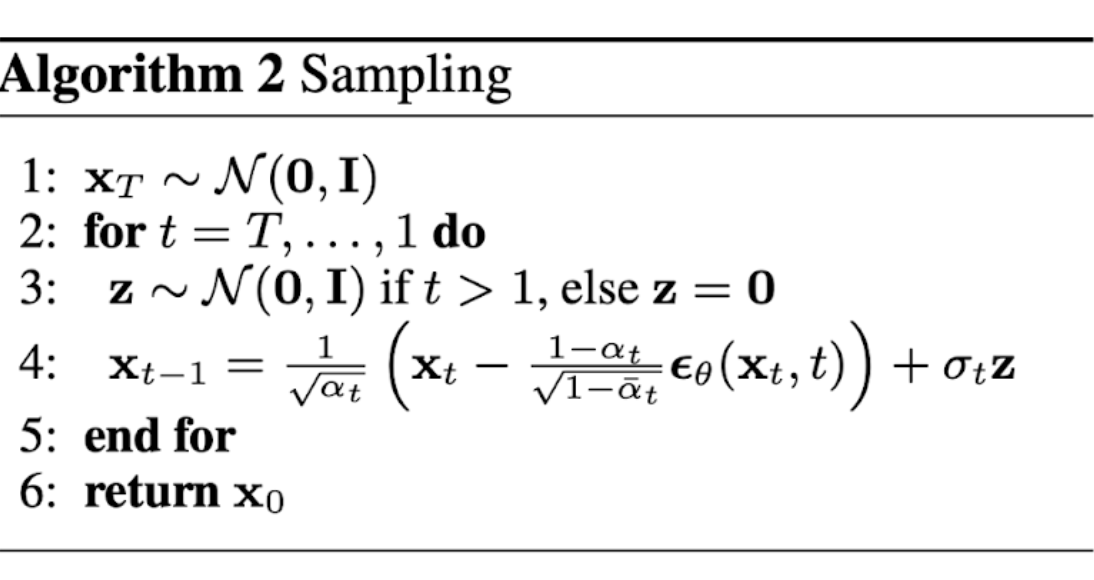
\includegraphics[width=8cm, keepaspectratio]{img/background_img/DDPM-sampling.png}
	\caption{Sampling algorithm \cite{weng2021diffusion}.}
\end{figure}
We start from $T$, where we sample pure noise from a Gaussian distribution, 
and then use the trained neural network to denoise it gradually at each time step until we end up at time step $t=0$.
Ideally, the algorithm will return an image coherent with the real data distribution.


\subsection{Stable Diffusion}\label{sec:stable-diffusion}
\emph{Stable Diffusion} \cite{rombach2022highresolution} changes the diffusion model architecture by making 
it a \emph{Latent Diffusion Model}. 
The training and the sampling are done in the \textbf{latent space}, 
a lower-dimensional representation of the image, giving the model a performance boost.
Stable Diffusion also accepts \textbf{textual prompts} as a conditioning input, making it a \emph{text-guided diffusion model}.

\subsubsection{The architecture}\label{sec:ldm-architecture} 

Fig. \ref{fig:ldm-architecture} shows the \textbf{architecture} of the Stable Diffusion model.
The first element is a VAE that transforms the \textbf{pixel space} of the input tensor into a latent space that is 
perceptually equivalent to the data space. The \emph{universal autoencoding stage} is trained before the DM, 
making it reusable on multiple DM trainings. A \emph{Transformer language model} $\tau_\theta$ is used as the language understanding component 
that takes the text prompt and produces \emph{token embeddings}. $\tau_\theta$ outputs 77 token embeddings vectors, each in 768 dimensions. 
The text representation is concatenated to the input tensor for diffusion, while all the generated tokens are mapped into the 
U-Net via the \emph{multi-head Attention}(Q, K, V) layers. The model still uses multiple \textbf{skip connections} and time step embeddings,
as in the pure Diffusion model.

\subsubsection{The Text Encoder}
The \emph{Transformer language model} used as the language understanding component inside the LDM is \emph{ClipText}, based on the OpenAI CLIP model.
CLIP stands for \textbf{Constastive Language-Image Pretraining} and is an open-source, multi-modal, zero-shot model. 
Given an image and text descriptions, the model can predict the most relevant text description for that image without 
optimizing for a particular task.


CLIP is trained on a 400 million image-text pairs dataset, and Fig. \ref{fig:clip-training} shows the training steps done for each 
data pair.
Firstly, each image and caption are encoded with an image and a text encoder. Then, using \emph{cosine similarity}, 
the two embeddings are compared to each other, giving a score that will be low at first. 
The two models get updated until the resulting embeddings are similar. 
After repeating these steps across the dataset with large batch sizes, the two encoders can produce \textbf{similar embeddings} 
for the correct image-text pairs. It is essential to notice that during the training process, 
the two models are also trained on \textbf{negative examples}, allowing the model to assign a low score to incorrect pairs.

\subsubsection{Classifier-free guidance}
During \textbf{inference}, instead of using a CLIP-guided diffusion method, Stable Diffusion uses 
\emph{classifier-free guidance} \cite{ho2022classifierfree}
that improves quality and decreases the sample diversity; 
this method also helps to emphasize the prompt input during diffusion. 
At each diffusion step, the model produces two images, one guided by text and one without access to the text. 
The difference between the two images is computed, scaled by the \textbf{CFG scale}, and then added to the text-less image, 
making the resulting image more faithful to the prompt. 
In conclusion, the CFG scale controls how much the diffusion process will be coherent with the prompt, 
so a lower CFG value will result in an image of higher quality but less faithful. Conversely, 
a higher value will result in a more coherent image but more distorted.

\subsubsection{Training}
The training process is similar to the one of the pure Diffusion model.
However, in this case, the loss function
uses the \textbf{latent data} $z_t=\sqrt{\bar{\alpha_t}}z_0 + \sqrt{1-\bar{\alpha_t}}\epsilon$ where
$z_0 = E(x_0)$ is the latent representation of the input image $x_0$.
In addition, the conditioning input $\tau_\theta(y)$ generated by the text encoder is also taken into account,
resulting in the following loss function:
\begin{equation}
	L_{LDM} = \mathbb{E}_{t,z_0,\epsilon,y}\left[||\epsilon-\epsilon_\theta(z_t,t,\tau_\theta(y))||^2\right]
\end{equation}

\subsubsection{Image to Image Diffusion}
Stable Diffusion is also able to generate an image from an \textbf{initial one}. This process, defined in multiple applications 
as ``\textbf{img2img diffusion}'', is done by applying \textbf{forward diffusion} to the input image for a certain amount of steps and then 
running the \textbf{backward diffusion} process on the noisy image until the model recovers a new one. A \textbf{noise strength} parameter 
that goes from 0.0 to 1.0, corresponds to what percentage of each noise step is added to the initial image. 
A higher parameter value will cause the diffusion process to deviate more from the original image, resulting in one with 
additional new details. 
In comparison, a lower noise strength value will cause the diffused image to be almost identical to the input one.

\subsection{ControlNet}
\emph{ControlNet} \cite{zhang2023adding} is a neural network architecture that can enhance 
pre-trained image diffusion models with task-specific conditions. 
The model manipulates the input conditions of network blocks to control the overall behavior of an entire neural network.


Fig. \ref{fig:controlnet}-(a) shows an arbitrary \textbf{neural network block} $\mathcal{F}(\cdot;\Theta)$, 
with a set of parameters $\Theta$,
where, for example, a \textbf{feature map} $x \in \mathbb{R}^{h\times w \times c}$, with ${h,w,c}$ 
being height, width, and channel numbers
is transformed into another feature map $y$ with
\begin{equation}
	y = \mathcal{F}(x;\Theta)
\end{equation}
In Fig. \ref{fig:controlnet}-(b), we can see how a ControlNet is applied to a neural network block.
All $\Theta$ parameters are locked and then cloned to a \textbf{trainable copy} $\Theta_c$, 
which is trained with an \textbf{external condition vector} $c$. 
This copy is created to avoid overfitting when the training dataset is small 
and to preserve the quality of large models. 
Finally, the two neural network blocks are connected via a \emph{zero convolution layer}, 
a $1\times1$ convolution layer with both weight and bias initialized as zeros.
By denoting the zero convolution operation as $\mathcal{Z}(\cdot;\cdot)$
and using two instances of parameters ${\Theta_{z1},\Theta_{z2}}$,
we can compose the ControlNet structure with
\begin{equation}
	y_c = \mathcal{F}(x;\Theta) + \mathcal{Z}(\mathcal{F}(x+\mathcal{Z}(c;\Theta_{z1});\Theta_c);\Theta_{z2})
\end{equation}
where $y_c$ is the output of the ControlNet block.
Thanks to the zero convolution layers, when ControlNet is applied to some neural networks block, 
it will not cause any changes to the deep neural features before optimization, resulting in $y=y_c$.
Next, the paper's authors show how having a zero convolution layer does not influence the weight 
and bias gradients as long as the condition vectors are non-zero, but the datasets ensure this.\\\\
``In this way, the 
zero convolutions become an unique type of connection layer that progressively grow from zeros to
optimized parameters in a learned way'' \cite{zhang2023adding}.\\


As shown in Fig. \ref{fig:controlnet-2}, ControlNet controls each level of the Stable Diffusion U-Net in a 
\textbf{computationally efficient} way due to the locked weights of the diffusion model, so no gradient computation on the original 
encoder is needed for training. With ControlNet, the overall learning objective becomes:
\begin{equation}
	L = \mathbb{E}_{z_0,t,c_t,c_f,\epsilon \sim \mathcal{N}(0,1)}\left[||\epsilon-\epsilon_\theta(z_t,t,c_t,c_f)||^2 \right]
\end{equation}
where $c_t$ are the text prompts and $c_f$ are task-specific conditions.
Here are all the types of conditioning available with ControlNet:
\begin{itemize}
	\item Canny edge.
	\item Hough line.
	\item HED boundary.
	\item User Sketching.
	\item Human pose (Openpose\footnote{Openpose github: \url{https://github.com/CMU-Perceptual-Computing-Lab/openpose}}).
	\item Semantic segmentation.
	\item Depth.
	\item Normal Maps.
	\item Cartoon Line Drawing.
\end{itemize}

\begin{figure*}[H]
	\centering
	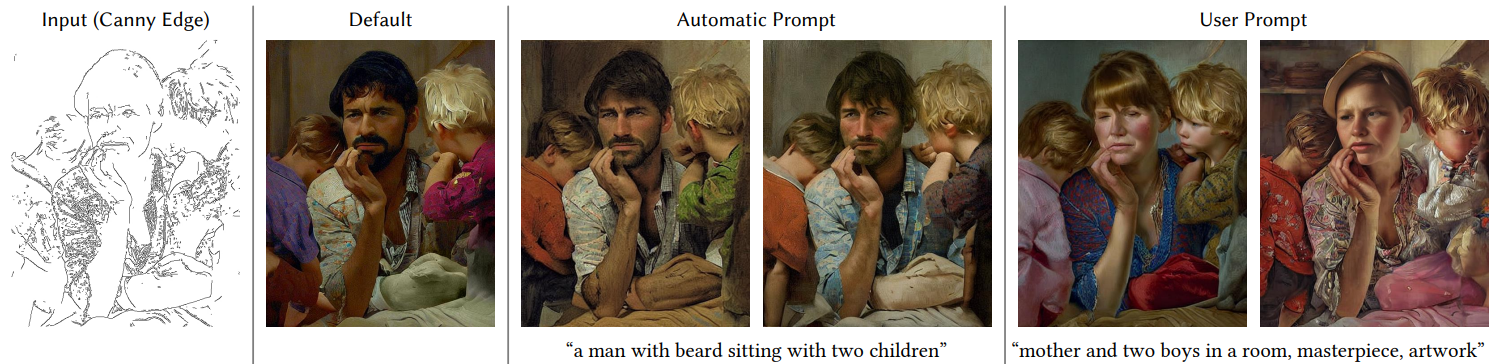
\includegraphics[width=15cm, keepaspectratio]{img/background_img/canny.png}
	\caption{Controlling Stable Diffusion with Canny edges \cite{zhang2023adding}.}
	\label{fig:canny}
\end{figure*}

Fig. \ref{fig:canny} shows how the \textbf{Canny edge conditioning} can be used to control the diffusion process,
resulting in new images with the same structure but different styles and subjects.
The automatic prompt was generated by BLIP based on the default image.

\subsection{LoRA (Low-Rank Adaptation)}
\emph{LoRA} \cite{hu2021lora} is a method that was firstly developed to adapt 
\emph{Large Language Models} (LLMs) to particular tasks or domains.\\ \\
``This method freezes 
the pre-trained model weights and injects \textbf{trainable rank decomposition matrices} 
into each layer of the Transformer architecture, greatly reducing the number of trainable 
parameters for downstream tasks'' \cite{hu2021lora}. \\\\
Some users started to use LoRA as an alternative to \emph{Dreembooth} \cite{ruiz2022dreambooth} 
and \emph{textural inversion} \cite{gal2022image} to 
fine-tune the Stable diffusion model. LoRA has some advantages over the other two techniques, 
resulting in small model files (2-200MBs), smaller than Dreembooth, 
while keeping an optimal result during diffusion. However, like textual inversion, 
a LoRA model must be used with a \textbf{SD model checkpoint file}.
In This case, LoRA applies small changes to the \textbf{cross-attention layers} by adding its 
weights to their weights matrices.
LoRA achieves a smaller file size by breaking its weight matrix into \textbf{two low-rank matrices}.
\begin{figure}[H]
	\centering
	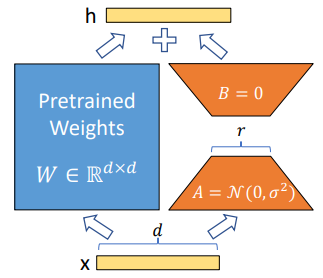
\includegraphics[scale=0.5]{img/background_img/LoRA.png}
	\caption{LoRA reparametrazation \cite{hu2021lora}.}
	\label{fig:lora}
\end{figure}
Fig. \ref{fig:lora} shows LoRA reparametrazation technique. Let us condiser a 
pre-trained weight matrix $W_0 \in \mathbb{R}^{d\times k}$, we can constrain its update
by representing it as a \textbf{low-rank decomposition} $W_0 = \Delta W=W_0+BA$, where $B \in \mathbb{R}^{d \times r}$,
$A= \in \mathbb{R}^{r \times k}$, and the rank $r \ll min(d,k)$.
During training, $W_0$ is frozen, wile $A$ and $B$ trainable parameters.
For $h = W_0x$, the forward pass yields:
\begin{equation}
	h = W_0x + \Delta Wx = W_0x + BAx
\end{equation}
$A$ is initialized to a random Gaussian and $B$ is initialized to zero, so that
$\Delta W = BA$ is zero.

\subsection{MediaPipe}
\emph{MediaPipe}\footnote{MediaPipe web page: \url{https://mediapipe.dev/}} 
is an open-source framework for building pipelines to perform computer vision 
inference over arbitrary sensory data such as video or audio.
MediaPipe offers the following solutions:
\begin{itemize}
	\item Face Detection.
	\item Face Mesh.
	\item Iris Detection.
	\item Hands Detection.
	\item Pose Detection.
	\item Holistic.
	\item Selfie Segmentation.
	\item Hair Segmentation.
	\item Object Detection.
	\item Box Tracking.
	\item Instant Motion Tracking.
	\item Objectron (3D).
	\item KNIFT.
	\item AutoFlip.
	\item MediaSequence.
	\item YouTube 8M.
\end{itemize}
But for this project, we will focus on the \emph{Face Detection} and \emph{Face Mesh} solutions.

\paragraph{Face Detection}


\emph{Face Detection} is a MediaPipe solution that \textbf{detects human faces} in an image or a video,
with six landmarks and multi-face support.
It is based on \emph{BlazeFace} \cite{bazarevsky2019blazeface}, a lightweight and well-performing 
face detector tailored for mobile GPU inference.
In Fig. \ref{fig:face-detection}, we can see how the BlazeFace pipeline is able to detect a face 
(highlighted with a red box) in an image, while the green points in the image are an example of a
\emph{task-specific model}.

\paragraph{Face Mesh}


\emph{Face Mesh} is a MediaPipe solution that estimates \textbf{468 3D face landmarks} in an image or a video,
by using machine learning to infer the \textbf{3d facial surface} without needing a dedicated depth sensor.
This ML pipeline consists of two real-time deep neural networks that work together.
The first one is a \textbf{detector} based on \emph{BlazeFace} that computes face locations on the full image.
The second is a \emph{3D face landmark model} \cite{kartynnik2019realtime} that operates on those locations and predicts the 
approximate 3D surface via regression. Fig. \ref{fig:face-mesh} shows some examples of face mesh predictions applied to two faces.


\subsection{Deepfakes}
\emph{Deepfakes} are an artificial intelligence technique that combines machine learning with computer graphics to create \textbf{fake videos or images that appear real}. 
The term “Deepfake” was first coined in late 2017 by a Reddit user of the same name. 
This user created a space on the online news and aggregation site where they shared pornographic videos that used open-source face-swapping technology.
Deepfakes use various generative models to analyze and learn from a large dataset of real images and videos and generate new ones remarkably similar to the original data.
This technology has been used to create realistic-looking videos of people doing things they never actually did or saying things they never actually said. 
For example, Deepfake videos have been created that show political leaders saying things they never actually said or celebrities in compromising or embarrassing situations.
While Deepfakes have some harmless uses, such as creating digital avatars for gaming and entertainment, they also pose a significant risk to society. 
Deepfakes can be used to spread disinformation and fake news, damage reputations, and even manipulate elections.

\subsubsection{Deepfakes with Autoencoders (AE) and Variational Autoencoders (VAE)} \label{sec:deep-vae}
We already introduced \emph{Autoencoders} \cite{bank2021autoencoders} in Section \ref{sec:vae}, 
but here we will go into further detail 
about how they can be used to create Deepfakes.
Their training is based on learning the functions $A : \mathbb{R}^n \rightarrow \mathbb{R}^p$ (encoder), 
and $B:\mathbb{R}^p \rightarrow \mathbb{R}^n$ (decoder), where both satisfy:
\begin{equation}
	arg~min_{A,B}E[\Delta(x,B \circ A(x))]
\end{equation}
where $E$ is the expectation over the distribution of $x$ and $\Delta$ is the reconstruction loss function (generally
$L_2$-norm), which measures the distance between the output of the decoder and the input.



This architecture commonly uses \textbf{multiple hidden layers} between the encoder and the decoder 
with fewer neurons than the number of input image pixels, creating a latent image representation. 
The generation of Deepfakes with AE consists of three significant steps.
First, an encoder is trained to produce feature maps for \textbf{both faces class}, while a decoder is trained as a \textbf{measure of encoder accuracy}. 
Then, as shown in Fig. \ref{fig:training-ae}, \textbf{two decoders are trained} separately to reproduce images from both classes. Finally, \textbf{decoders are switched} to produce
images from one class based on feature maps from the other, illustrated in Fig. \ref{fig:generation-ae}.
This same method can be applied to generate Deepfakes with VAE (Section \ref{sec:vae}), the only difference being \textbf{how the latent
	vector is obtained}.

\subsubsection{Deepfakes with VAE/GAN}
\begin{figure}[H]
	\centering
	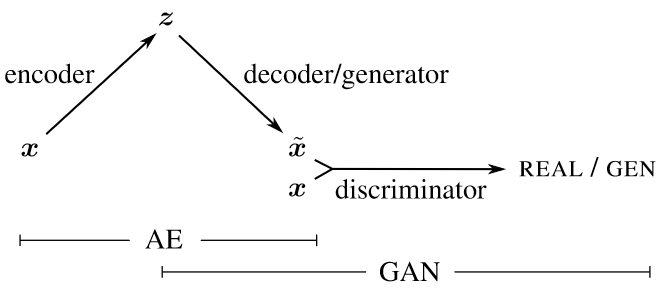
\includegraphics[scale=0.35]{img/background_img/vae-gan.png}
	\caption{VAE/GAN network \cite{larsen2016autoencoding}.}
	\label{fig:vae-gan}
\end{figure}
\emph{VAE/GAN} \cite{larsen2016autoencoding} is a combination of \emph{Variational Autoencoders} and \emph{Generative Adversarial Networks}
that leverages learned representations to better measure similarities in data space.
Fig. \ref{fig:vae-gan} shows how it is possible to combine a VAE with a GAN by \textbf{collapsing} the VAE decoder and the GAN generator 
into one and then letting them share parameters and training them jointly. 
This unsupervised generative model simultaneously learns to encode, generate, and compare datasets samples. 
The method used to generate Deepfakes is similar to the one explained in Section \ref{sec:deep-vae} while achieving 
better results by leveraging the GAN discriminator.



















\section{Project} \label{ch:project}
In this chapter, we will see how all the technologies presented in the previous 
chapter can be used to create an application to generate Deepfakes through Stable Diffusion. 
Starting from how the input video needs to be processed. 
We will then understand how we can use LoRA and Stable Diffusion with ControlNet to 
generate images of a target subject and how these images can be applied to the input video, 
creating a real Deepfake. 
Finally, we will understand the problems of this process and how they can be improved.
\subsection{Infographic} \label{sec:project_info}
\begin{figure}[H]
	\centering
	\includegraphics[width=1.1\textwidth, keepaspectratio]{img/project_img/infografica.png}
	\caption{The entire pipeline used to create Deepfakes.}
	\label{fig:project}
	
	
\end{figure}
In Fig. \ref{fig:project}, we can see the entire \textbf{pipeline} used to create Deepfakes from a video source. 
First, the input video is decreased to 12 frames per second. 
Then for every frame, by using \emph{MediaPipe}, we can extrapolate face locations and their structure. 
Next, the structure created with \emph{Face Mesh} is processed to create a mask for the latter application of the diffused image, 
while the locations detected by \emph{Face Detection} are used to extract just the face.
After this, every cropped image is processed through \emph{Stable Diffusion} with \emph{ControlNet} and \emph{LoRA}. 
This LoRA model was previously trained to the target face in a process that will be further explained in Section \ref{sec:lora_training_webui}. 
Finally, every diffused image gets applied to the corresponding input frame and then exported as a video. 
In the following sections, we will further elaborate on every step of this process. 

\subsection{Video Preprocessing} \label{sec:video_preprocessing}

\subsubsection{Decreasing Frame Rate} \label{sec:decreasing_frame_rate}

\begin{figure}[H]
	\centering
	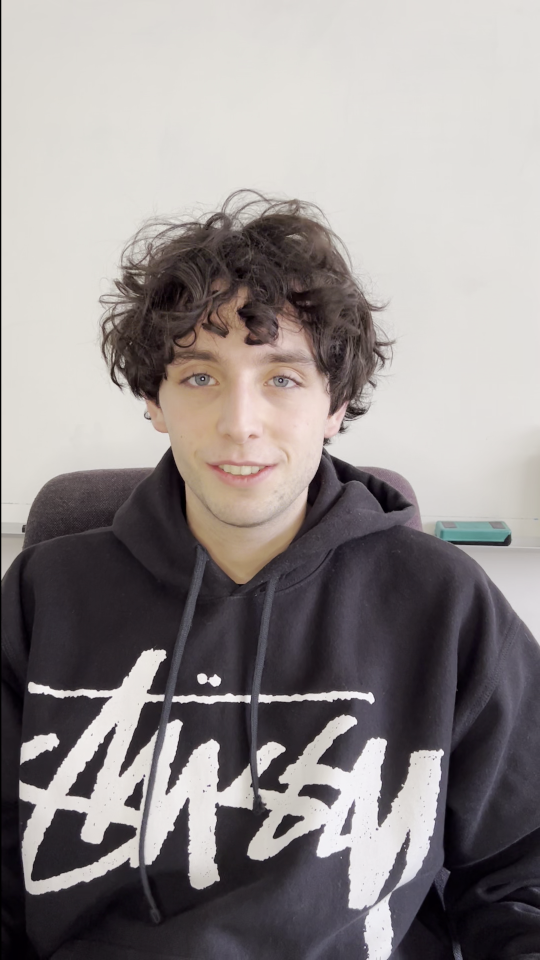
\includegraphics[scale=0.2, keepaspectratio]{img/project_img/init.png}
	\caption{Example of an input frame.}\label{fig:init-frame}
\end{figure}


The first step of the \textbf{preprocessing pipeline} is decreasing the frame rate to \textbf{12 FPS}. 
This processing saves time later during the diffusion phase, having fewer frames to work on. 
Twelve frames per second is the frame rate used in all major animation studios to ensure the minimum number of 
frames while maintaining fluidity in a video. A python library called \emph{OpenCV}\footnote{OpenCV website: \url{https://opencv.org/}} 
was used to achieve this goal. 
First, a function called ``\textbf{get-saving-frames-durations}'' returns the list of durations where to save the frames; 
this is done by creating a list of evenly spaced time points from $t=0$ to the end of the video, with a step of $1/12$. 
After this, the primary function extracts the earliest saving time from the list of durations; 
If this one is less than or equal to the current frame duration, calculated by dividing the frame counter by the original FPS, 
then the current frame gets saved, and the frame counter increases. This iterative process stops when the list of durations is empty, 
resulting in the desired frame rate. In Figure \ref{fig:init-frame}, we can see an example of a frame from the input video.
This frame will be used as a base for all the following examples.



\subsubsection{Face Detection and Face Mesh} \label{sec:face_detection}

\begin{figure}[H]
	\centering
	\begin{subfigure}[b]{0.5\textwidth}
		\centering
		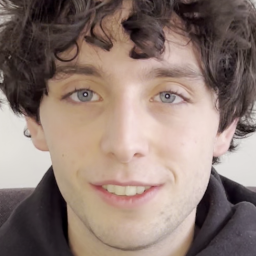
\includegraphics[width=4cm, keepaspectratio]{img/project_img/cropped.png}
		\caption{Cropped frame.}\label{fig:cropped}
	\end{subfigure}%
	\hfill
	\begin{subfigure}[b]{0.5\textwidth}
		\centering
		
\includegraphics[width=4cm, keepaspectratio]{img/project_img/mask-blur.png}
		\caption{Face mask.}\label{fig:mask}
	\end{subfigure}
	\caption{Outputs from MediaPipe preprocessing.}\label{fig:project-mediapipe}
\end{figure}


The next step is to crop just the face. 
This decision is to help Stable Diffusion stay \textbf{consistent} through every frame during diffusion since the noise added is the same, 
resulting in a similar output for each frame (\textbf{the seed is locked}). 
In addition, the decrease in image size also helps reduce the time needed for diffusion. 
To achieve this result, we use \emph{MediaPipe Face Detection} that, given an input frame, 
returns a \textbf{proto message} that contains a \textbf{bounding box} and \textbf{six key points} (right eye, left eye, nose tip, mouth center, right ear tragion, and left ear tragion). 
The bounding box is composed of $xmin$ and $width$ by $ymin$ and $height$, all normalized to [0.0,1.0]. 
At the same time, each key point is composed of $x$ and $y$, which are also normalized to [0.0,1.0] by the image width and height, respectively. 
Since the bounding box is right on the face, a \textbf{padding of 30 pixels} was added to ensure a full face capture.
Then all the bounding box points get saved to a \emph{PKL file} for later use. 
An example of a cropped frame can be seen in Fig. \ref{fig:cropped}.
After cropping, all the images are resized to $512 \times 512$ to ensure further \textbf{coherence} during diffusion. 
The next step is to compute the face mask. 
This is done through \emph{MediPipe Face Mesh} that, given an input frame, returns a list of \textbf{468 face landmarks} 
where each landmark is composed of $x$, $y$, and $z$, all normalized to  [0.0, 1.0]. 
Next, we must find the \emph{convex hull} of all the returned landmarks to locate the face mask points, considering only the $x$ and $y$ coordinates. 
This was done with \emph{Graham's scan algorithm} \cite{GRAHAM1972132} that works in $O(n log n)$ time. Let us consider an array of $n$ points, following is Graham's scan algorithm:
\begin{enumerate}
	\item Find the point with the lowest $y$ coordinate, breaking ties by choosing the point with the lowest $x$ coordinate. 
	Let this point be $P_0$. Put $P_0$ at first position in the output hull.
	\item Consider the remaining $n-1$ points and sort them by polar angle in counterclockwise order around $P_0$.
	\item Check if two or more points have the same polar angle. If so, remove all except the one that is farthest from $P_0$. 
	Let the size of the remaining set of points be $m$.
	\item If $m \leq 2$, the algorithm terminates; the convex hull is not possible.
	\item Create an empty stack $S$ and push $P_0$, $P_1$, and $P_2$ to it.
	\item Process the remaining $m-3$ points one at a time, starting from $P_3$. by doing:
	\begin{enumerate}
		\item Keep removing points from $S$ while the orientation of topmost point, next-to-top point, and current point is not counterclockwise.
		\item Push the current point to $S$.
	\end{enumerate}
	\item The points in $S$ are the output convex hull.
\end{enumerate}

\begin{figure}[H]
	\centering
	\begin{subfigure}[b]{0.5\textwidth}
		\centering
		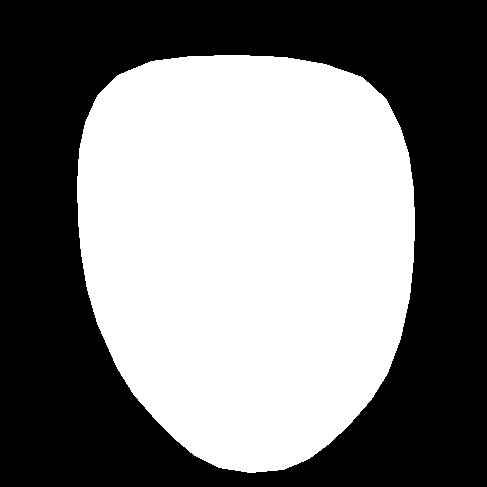
\includegraphics[width=4cm, keepaspectratio]{img/project_img/mask.png}
		\caption{Mask without processing.}\label{fig:mask-noblur}
	\end{subfigure}%
	\hfill
	\begin{subfigure}[b]{0.5\textwidth}
		\centering
		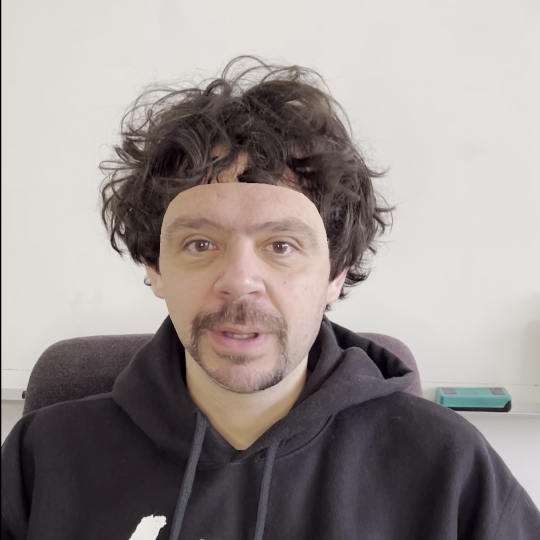
\includegraphics[width=4cm, keepaspectratio]{img/project_img/final-erorr.png}
		\caption{The output with the same mask.}\label{fig:mask-final-error}
	\end{subfigure}
	\caption{Mask and its application without processing.}\label{fig:eroor-mediapipe}
\end{figure}


After finding the convex hull, we can draw a white polygon on a black background corresponding to the \textbf{face mask}, 
and an example can be seen in Fig. \ref{fig:mask-noblur}. 
This image can be used to do \emph{soft masking} of the diffused image by making transparent all 
pixels corresponding to a black pixel on the mask. 
The problem with applying this mask is that it would result in a \textbf{detectable compositing} due to the straight borders, 
as we can see in Fig. \ref{fig:mask-final-error}. 
To solve this problem, we need to smooth all the borders of the mask. 
This was done through multiple steps of \textbf{erosion} and \textbf{Gaussian blur}, 
resulting in a mask with smooth borders that can be seen in Fig. \ref{fig:mask}.

\subsection{Stable Diffusion WebUI} \label{sec:stable_diffusion_webui}


A browser interface based on \emph{Gradio library}\footnote{Gradio website: \url{https://gradio.app/}} 
created by AUTOMATIC1111\footnote{Stable Diffusion WebUI github: \url{https://github.com/AUTOMATIC1111/stable-diffusion-webui}} 
(Fig. \ref{fig:webui}) 
was used to operate Stable Diffusion. 
This interface offers all Stable Diffusion modules optimized for \textbf{lower VRAM usage}, down to 2GB. 
The software creates a \textbf{local server on port 7860} and, 
using the \emph{Xformers library}\footnote{Xformers github: \url{https://github.com/facebookresearch/xformers}} 
further speeds up the image generation process on \textbf{Nvidia GPUs}.
The most exciting part is that this software offers an extension module to 
implement ControlNet and LoRA models with just a click. 
To call a LoRA model for diffusion, we need to write in the prompt ``\textbf{<lora:ModelName:$\alpha$>}'', 
where ModelName is the name of the model file without the extension, 
and $\alpha$ is the weight applied to the LoRA model that goes from 0 to 1 (with 0 the model is disabled). 

Given that the application developed for this project is standalone, 
we need a way to communicate with the web UI. We can use the \emph{API}  (shown in Fig. \ref{fig:api}) 
the local server offers for this.
We can communicate with the Stable Diffusion web UI through simple 
POST and GET requests through an \textbf{HTTP communication}. 
\begin{python}
	payload = {
		"init_images": [
		b64_img(image)
		],
		"prompt": prompt,
		"negative_prompt": negative_prompt,
		"steps": steps,
		"width": image.width,
		"height": image.height,
		"seed": seed,
		"cfg_scale": cfg_scale,
		"denoising_strength": denoising_strength,
		"sampler_index": "Euler a",
		"controlnet_units":[
		{
			"module": "canny",
			"model": "control_canny-fp16 [e3fe7712]",
		}
		]
	}
\end{python}
The \textbf{JSON payload} used for diffusion is composed of several elements.
First, we have an array of images to diffuse (in our case, just one image), 
where each image is encoded to \textbf{Base64}. 
Then, we have the conditioning parameters, \textbf{prompt} and \textbf{negative prompt}, 
that tell Stable Diffusion what and what not to generate during the diffusion process. 
The \textbf{steps} represent the number of diffusion steps needed, while \textbf{width} 
and \textbf{height} are the dimensions of the output image. 
The \textbf{seed} parameter is used for the Gaussian noise and is generally fixed to the same value. 
The \textbf{CFG scale} is used for \emph{Classifier-free guidance} during diffusion, 
and the denoising strength tells Stable Diffusion how much noise to put on the input image. 
The \textbf{sampler index} indicated which sampler to use; in our case, ``Euler a'', 
which is the one that gave better results during testing.
Ultimately, the \textbf{controlnet units} represent which preprocessing module and model to use with ControlNet.
This payload is then sent to ``\textbf{127.0.0.1:7860/controlnet/img2img}'' for processing. 
The \textbf{response} is composed of two images, the first one is the image generated with Stable Diffusion, 
and the second one is the result of the ControlNet canny preprocessing of the input image.
\subsection{LoRA Training WebUI} \label{sec:lora_training_webui}
\begin{figure}[H]
	\centering
	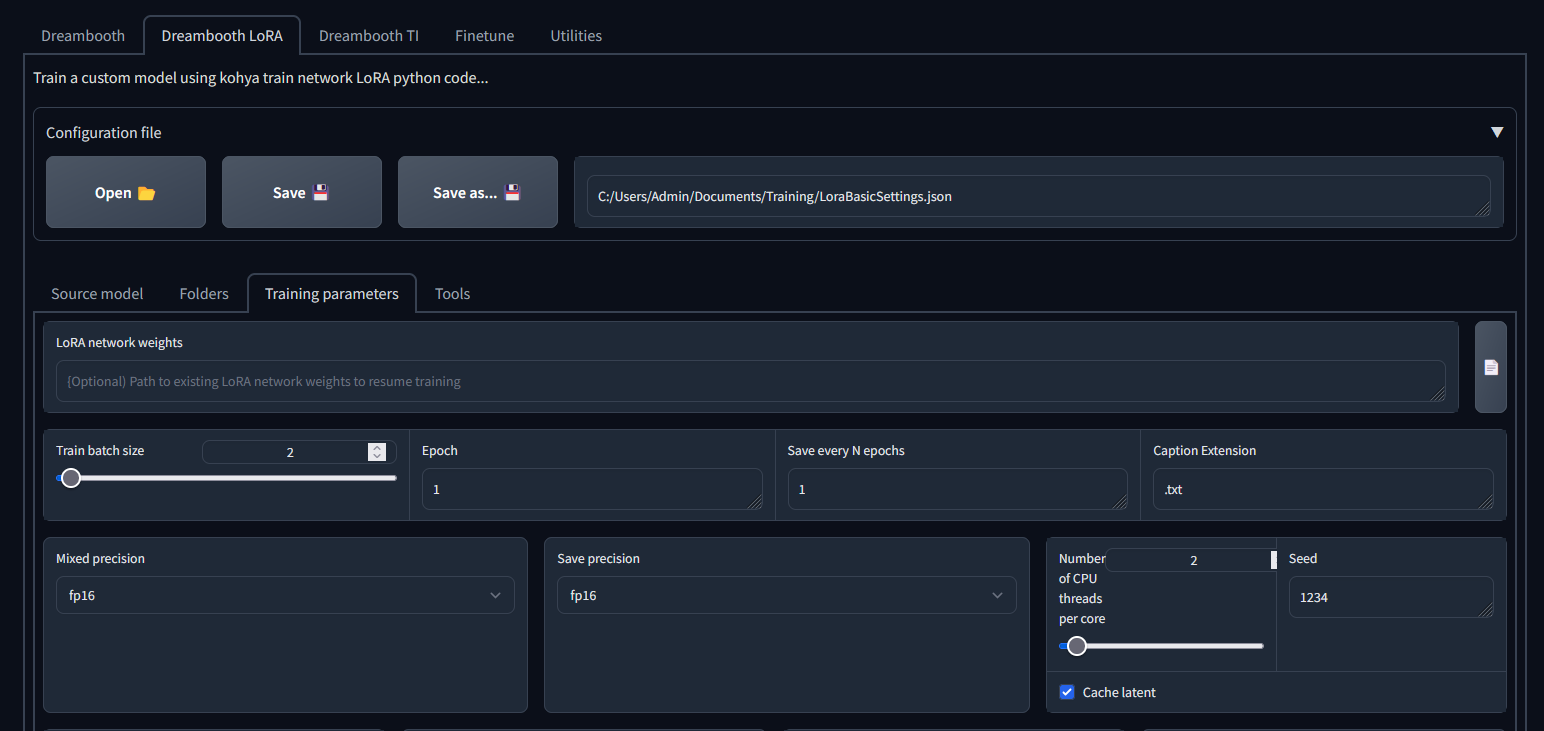
\includegraphics[width=15cm, keepaspectratio]{img/project_img/lora.png} 
	\caption{LoRA training webUI.}
	\label{fig:lora-webui}
\end{figure}
To train a LoRA model, a \emph{Windows-focused Gradio GUI}\footnote{Kohya webui github: \url{https://github.com/bmaltais/kohya_ss}}
(shown in Fig. \ref{fig:lora-webui}) 
for \emph{Kohya's Stable Diffusion trainers}\footnote{Kohya ss scripts github: \url{https://github.com/kohya-ss/sd-scripts}} was used. 
The GUI allows us to set the training parameters and run the required 
CLI commands to train the model with just \textbf{7GB of VRAM}. 
The first step is to prepare the dataset. For this purpose, 
a video of the target subject doing \textbf{multiple facial expressions} in \textbf{different lighting conditions} 
is required. In our case, a 2-minute video of professor Francesco Santini was recorded with a phone. 
The 60 FPS video was then lowered to \textbf{30 FPS}, and with \emph{MediaPipe Face Detection},
the face was extracted from all the frames in the same way proposed in Section \ref{sec:face_detection}.
Having the model trained on a dataset of $512\times 512$ images similar to the input images 
of the diffusion process helps us achieve a more consistent result in the end. 
Then we need to eliminate all the blurred images from the dataset. 
To perform \emph{blur detection}, we can use the \emph{variance of the Laplacian} \cite{903548}. 
This simple method can be implemented with just a single line of code with the help of OpenCV. 
First, we convolve a single channel of the input image with the \emph{Laplacian kernel}:
\begin{equation}
	\begin{bmatrix}
		0 & 1 & 0\\
		1 & -4 & 1\\
		0 & 1 & 0
	\end{bmatrix}
\end{equation}
Furthermore, we take the response's variance (i.e., standard deviation squared) 
and compare it to a \textbf{pre-defined threshold}; if it falls below, the image is blurry; otherwise, it is not.
The Laplacian operator is generally used to measure the second derivative of an image, 
highlighting regions containing rapid intensity changes. 
We can affirm that if the image contains a high variance, there is a wide spread of responses, 
representing an in-focus image. Opposingly, a  low variance represents a small spread of responses, 
indicating few and small edges, a clear sign of blur.
Now that we have eliminated all the blurry images, 
we must pair each frame with a textual description before training. 
We do not want to do this process by hand for all the dataset. 
Instead, we can use \emph{Bootstrapping Language-Image Pre-training} (BLIP) captioning \cite{li2022blip} 
to generate all the captions for us. 

\begin{figure}[H]
	\centering
	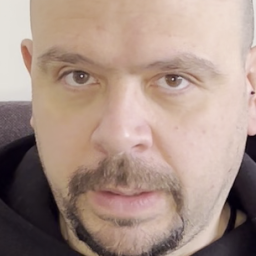
\includegraphics[scale=0.3, keepaspectratio]{img/project_img/santini-training.png}
	\caption{Sample from the training dataset.}
	\label{fig:santini-training}
\end{figure}


We take as an example Fig. \ref{fig:santini-training}, 
and then BLIP captioning generates the following caption 
where we add the name of our target subject as an \textbf{identifier} at the start:\\\\
``Francesco Santini a bald man with a beard and a black shirt''\\\\
We are now ready to start the training process. 
First, all the parameters for training are set with a JSON file generated by the main application 
(further explained in Section \ref{sec:gui}), 
so we just need to press a button. 
The training, for a small dataset of around a thousand images, 
takes about 4 hours on a machine mounting an Nvidia RTX 3070 Ti with 8 GB of VRAM. 
The result is a 200 Mb \emph{SafeTensors file} (our model) 
that needs to be added to the Stable Diffusion web UI and is now ready for diffusion.

\subsubsection{Custom Light}


As said before, during the creation of the training dataset, we need to have multiple 
light conditions for our target subject. 
Therefore, a custom light was developed to obtain this result in a controlled way.
This light, shown in Fig. \ref{fig:light}, is constructed with recycled materials.
The external wood frame comprises two picture frames fixed with nails to ensure stability. 
In addition, one glass plate is used as an insulator to separate the LEDs from the aluminum refractor.
The other plate, modified with two layers of plastic light diffusers, 
decreases the light intensity, making it a \textbf{soft light}.
The handle is part of a pipe clamp glued on top to make the light easier to hold.

\begin{figure}[H]
	\centering
	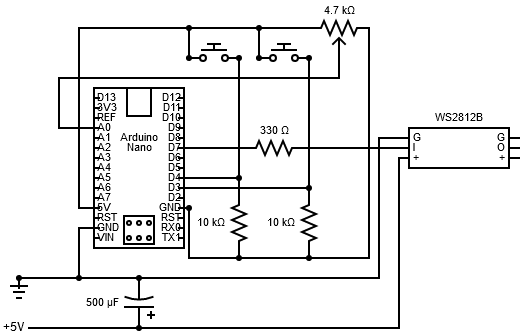
\includegraphics[scale=0.5, keepaspectratio]{img/project_img/circuit-light.png}
	\caption{The circuit.}
	\label{fig:light-circuit}
\end{figure}

The light is generated by an array of 100 RGB LEDs (WS2812B) that need a 5V, 50W external power supply. 
The circuit is shown in Fig. \ref{fig:light-circuit} and helps us understand how the light works. 
First, an \emph{Arduino Nano} controls all the logic and has its own power supply. 
Next, the board is connected via a digital pin to the LED strip and is protected 
from \textbf{signals reflections} by a $330\Omega$ resistor. 
A $500 \mu F$ capacitor is used on the LED powerline to help provide current 
while the power supply adjusts to the \textbf{varying load demands}. 
Since we also need a signal return for the LED data pin, the board's ground was 
connected to the power supply's ground. 
Finally, two buttons and one potentiometer are connected to the Arduino Uno to give tactile 
control over the light. 
The potentiometer controls the intensity of the light, 
while the two buttons give us access to a menu. 
The first button cycles through two states, ``\textbf{static light mode}'' and ``\textbf{light cycle mode}''. 
With static light, we get a fixed color that can be changed with the second button. Instead, 
with the light cycle mode, we get a perpetually changing color, 
where the second button controls how fast the cycle is.



\subsection{Image Generation}

\begin{figure}[t]
	\centering
	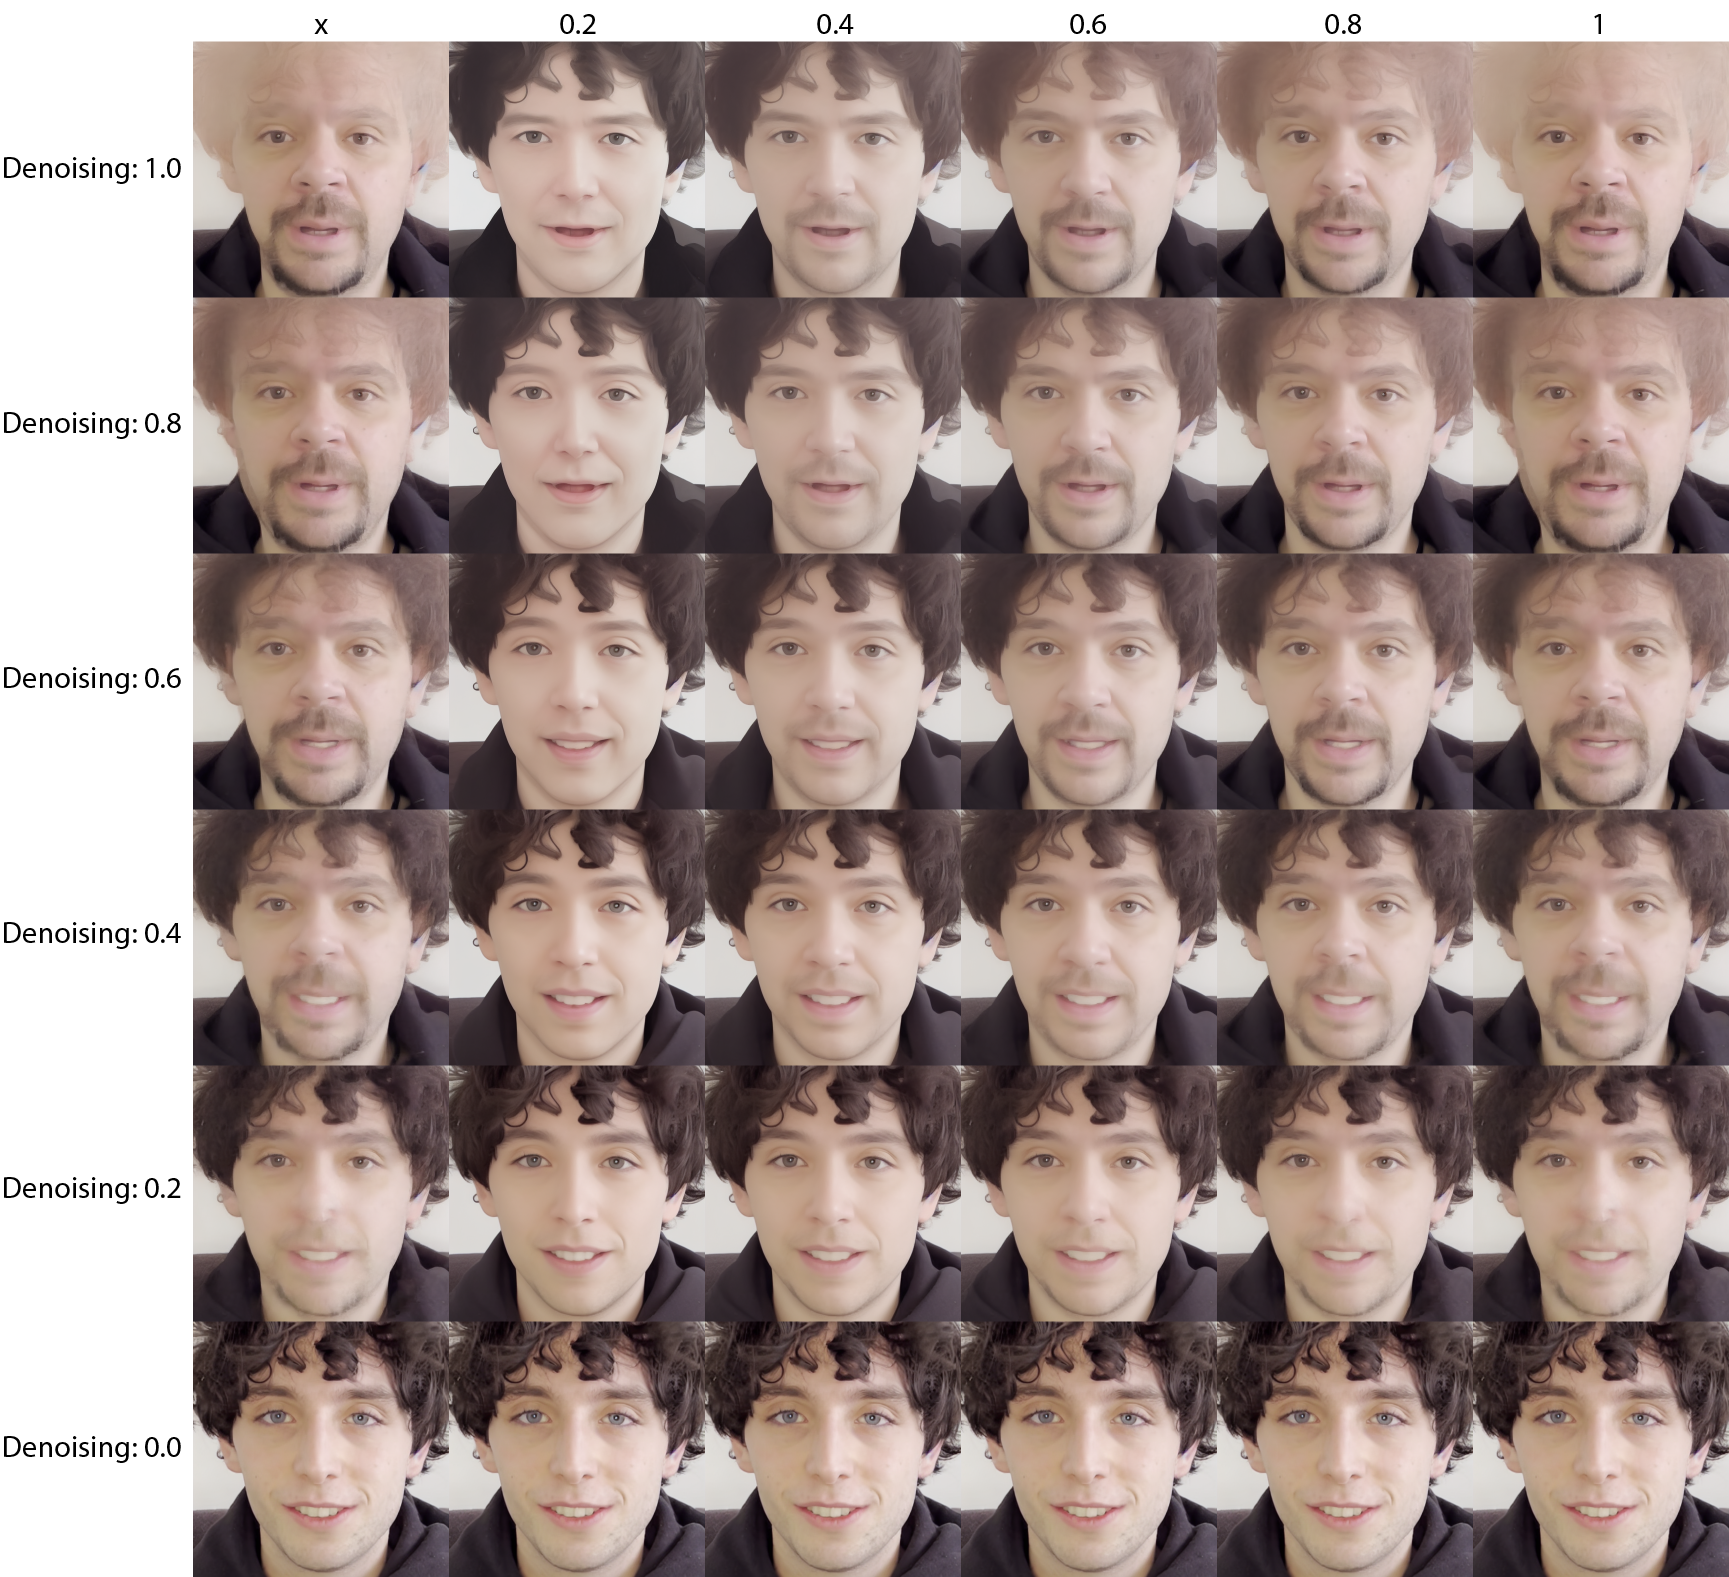
\includegraphics[scale=0.2, keepaspectratio]{img/project_img/grid-santini.png}
	\caption{Effects of Denoising and weight of a LoRA model on diffusion.}
	\label{fig:grid-santini}
\end{figure}


As seen in Section \ref{sec:stable_diffusion_webui}, the image generation process is done through 
a local server running Stable Diffusion. 
It takes about \textbf{15 seconds} for each $512 \times 512$ image. 
The main software offers the possibility to test the various parameters 
on just one image and, when ready, apply them to all the images. 
These parameters define how the process is going to happen.
First, we have the \textbf{prompt} that needs to describe what face we want, or in the case of LoRA, 
which model to use.
Then, a \textbf{negative prompt} is used to further condition the diffusion by 
describing what we do not want to see in the final image. 
For example, in our case, the negative prompt was:\\\\
``Distorted eyes, distorted mouth, distorted face, blue eyes, distorted teeth''\\\\
The number of \textbf{diffusion steps} will result in a less detailed image with lower values and 
a more detailed image with higher values. 
It is essential to notice that a high number of steps will result in the model 
``hallucinating'' too many details, distorting the final image.
In Fig. \ref{fig:grid-santini}, we can see how the \textbf{denoising strength} (on the left) 
and the \textbf{$\alpha$ parameter} (on top) of the LoRA model affect the diffusion. 
The denoising strength describes how much the final image will resemble the original one, 
while $\alpha$ indicates the weight of the LoRA model. 
Of course, there are no correct values to use, but through testing, 
a denoising strength of 0.4 and an $\alpha$ of 1 were optimal for
Deepfake generation when a LoRA model is used. 
\begin{figure}[H]
	\centering
	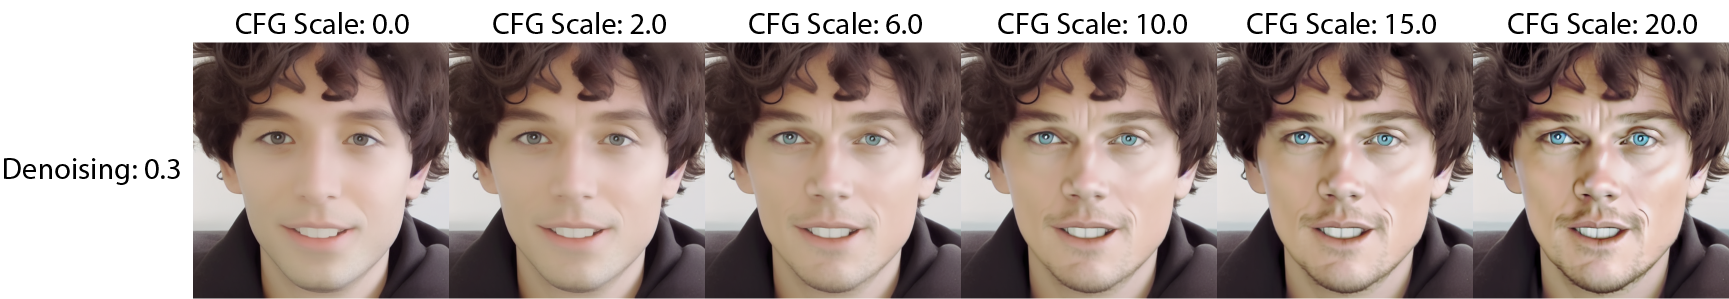
\includegraphics[width=\textwidth, keepaspectratio]{img/project_img/cfg-examples.png}
	\caption{How the CFG scale affects the image generation.}
	\label{fig:cfg-examples}
\end{figure}
If we did not use a LoRA model and instead a pure Stable Diffusion model, 
it is crucial to consider the \textbf{CFG scale}. 
This parameter indicates how much the diffusion process will adhere to the prompt. 
For example, in Fig. \ref{fig:cfg-examples}, we can see how it affects the final image. 
Like the number of steps, a higher value will result in a distorted output. 
However, a lower value will not affect the original image resulting in an almost identical output. 
Through testing, the optimal CFG scale value was around 7.

\begin{figure}[H]
	\centering
	\begin{subfigure}[b]{0.5\textwidth}
		\centering
		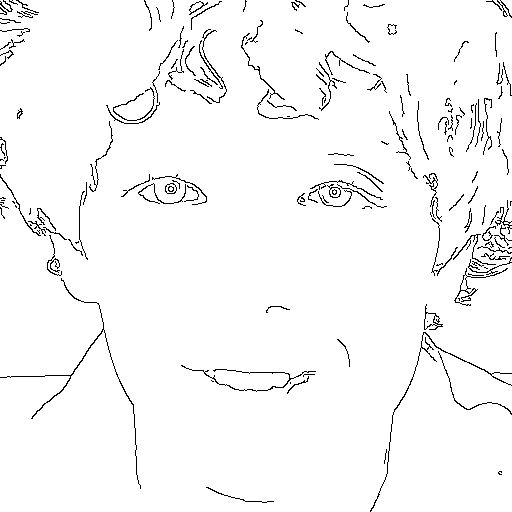
\includegraphics[scale=0.2]{img/project_img/canny.png}
		\caption{Correct canny.}\label{fig:canny-project}
	\end{subfigure}%
	\hfill
	\begin{subfigure}[b]{0.5\textwidth}
		\centering
		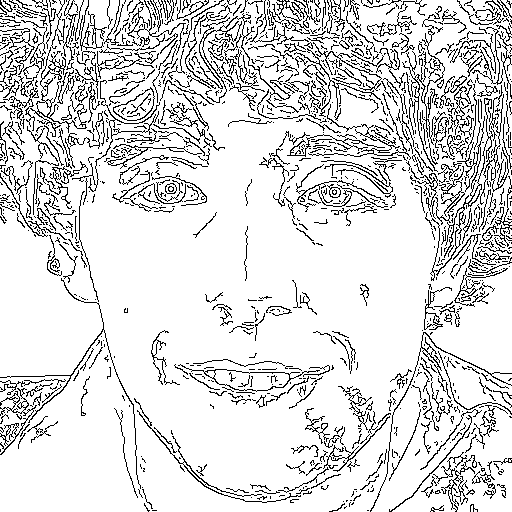
\includegraphics[scale=0.2]{img/project_img/canny-error.png}
		\caption{Incorrect canny.}\label{fig:canny-error}
	\end{subfigure}
	\caption{Examples of canny preprocessing.}\label{fig:canny-examples}
\end{figure}


The final thing to consider is the \textbf{ControlNet canny preprocessing}. 
The canny preprocessing is controlled through a low threshold and a high threshold. 
Unfortunately, at the time of writing this paper, there are no ways of 
controlling these two through the API.
Our objective, in this case, is to obtain an image similar to Fig. \ref{fig:canny-project}, 
where essential parts like mouth, nose shape, and eyes are highlighted without too many details. 
Furthermore, this image will produce an optimal and consistent generation through each frame, 
further helping to resolve the non-deterministic behavior of Stable Diffusion.
Differently,  an image similar to Fig. \ref{fig:canny-error} will have too many details to be computed, 
resulting in a distorted output.



\subsection{Deepfake and Video}
\begin{figure}[H]
	\centering
	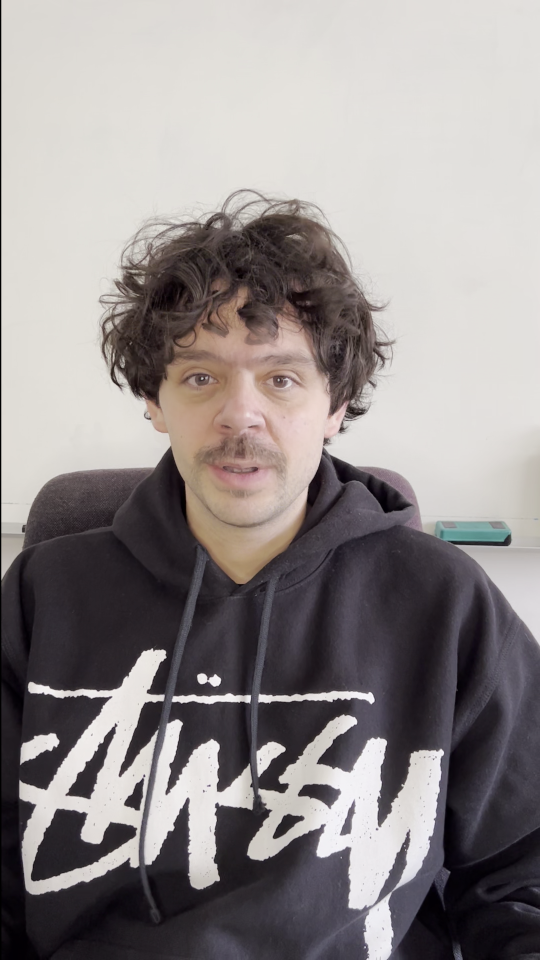
\includegraphics[scale=0.2, keepaspectratio]{img/project_img/output.png}
	\caption{Example of an output frame.}
	\label{fig:output}
\end{figure}
The final step of this process is to apply the diffused images to the initial frames 
and then create the final video. 
To complete this process, the software cycles through all the \textbf{diffused images} 
and finds the corresponding \textbf{initial frame} and \textbf{mask} for each one. 
Then, to find where to apply them, the software utilizes the \emph{PKL file} 
containing all the original bounding box sizes and locations. 
First, the image gets resized to its original size and then pasted 
to its correct position on the initial frame with its mask. 
An example of a final frame can be seen in Fig. \ref{fig:output}.
Ultimately, all the final frames get united into a single \textbf{12 FPS AVI file} with the help of OpenCV.

\subsection{GUI} \label{sec:gui}
The GUI was developed with \emph{PyQt6}\footnote{PyQt6: \url{https://pypi.org/project/PyQt6/}}, 
a Python library for creating GUI applications using the \emph{Qt toolkit}. 
The application comprises a \textbf{600 x 900 pixels main window} where a \textbf{tab menu} gives users access to each page.
All the pages utilize \emph{QtWidgets} to create the graphical components, 
while a \textbf{thread worker} does all the heavy calculations and communicates 
with the components through \textbf{signals}. 
This structure allows the user to interrupt every process while it is running.
For the purpose of this application, a \textbf{custom QtWidget} 
was developed to show each step of the processing as an image dynamically. 
Following are the descriptions of each page.
\subsubsection{File Menu Window}

\begin{figure}[H]
	\centering
	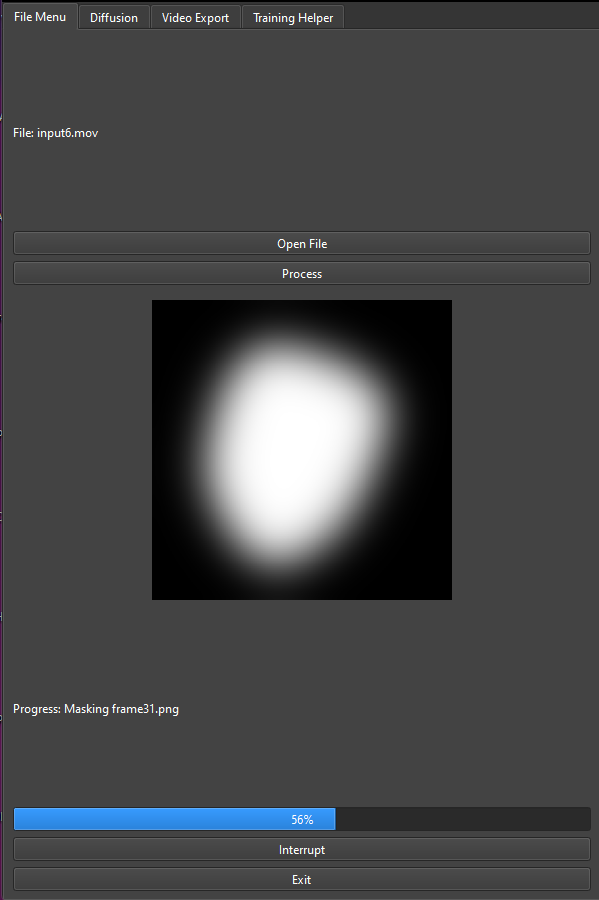
\includegraphics[scale=0.35, keepaspectratio]{img/project_img/file-window.png}
	\caption{The file menu window.}
	\label{fig:file-menu}
\end{figure}


The file menu (Fig. \ref{fig:file-menu}) lets users choose which video file to process through 
an ``\textbf{Open File}'' button. 
The ``\textbf{Process}'' button starts the preprocessing explained in section \ref{sec:video_preprocessing}, 
while the custom QtWidget shows each step. 
A \textbf{label} showing the current file being processed with a corresponding \textbf{progress bar} 
was employed to display the overall progress explicitly. 
The ``\textbf{Interrupt}'' button allows the user to interrupt the preprocessing. 
Finally, the ``\textbf{Exit}'' button closes the application and cleans all the generated data. 
After the preprocessing, the user gets redirected to the next tab,
where it is possible to use Stable Diffusion. 



\subsubsection{Diffusion Window}

\begin{figure}[H]
	\centering
	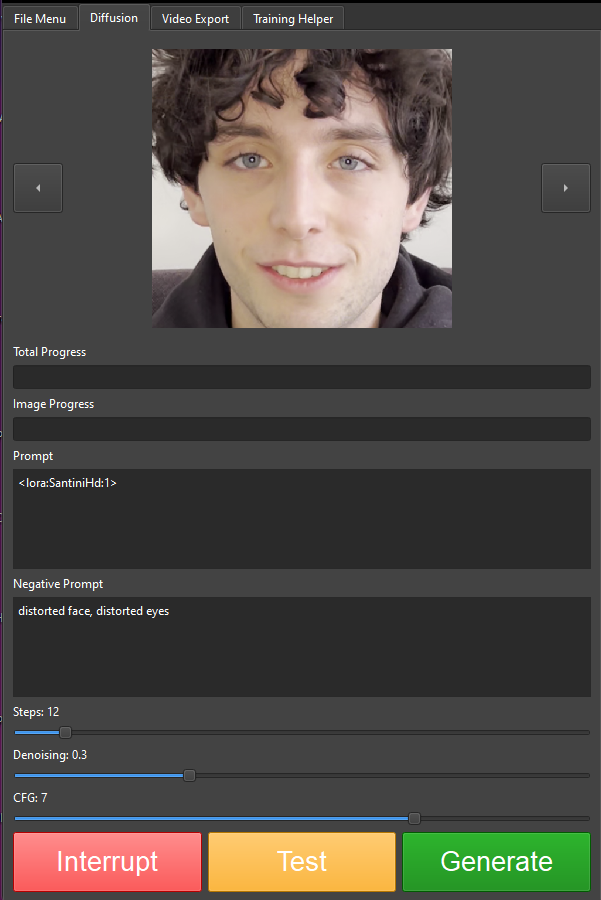
\includegraphics[scale=0.4, keepaspectratio]{img/project_img/generation-window.png}
	\caption{The diffusion window.}
	\label{fig:diffusion-menu}
\end{figure}



The diffusion window (Fig. \ref{fig:diffusion-menu}) comprises an \textbf{image viewer} that 
shows the cropped frames, where each frame can be cycled with the two \textbf{side buttons}. 
The \textbf{two progress bars} respectively indicate the overall and 
specific progress (testing, diffusion, frame application, and video generation). 
\textbf{Two text boxes} allow the users to input the prompt and the negative prompt, 
while \textbf{three sliders} are used to input steps, denoising strength, and CFG scale. 
The ``\textbf{Test}'' button tests Stable Diffusion parameters onto a single frame chosen 
in the upper part, and the result is shown in the same image viewer. 
The ``\textbf{Generate}'' button starts the complete process by collapsing the widgets used 
for the parameters input and then showing each step, from diffusion to video generation, 
in the image viewer. 
Finally, the ``\textbf{Interrupt}'' button allows the user to interrupt the processing. 
After the video is generated, the user gets redirected to the video export tab.

\subsubsection{Video Export Window}

\begin{figure}[H]
	\centering
	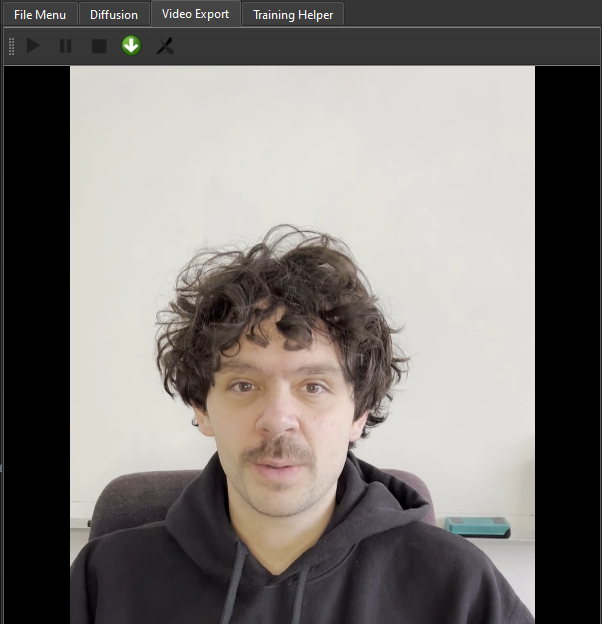
\includegraphics[scale=0.3, keepaspectratio]{img/project_img/video-window.png}
	\caption{The video export window.}
	\label{fig:video-player}
\end{figure}

The video export window (Fig. \ref{fig:video-player}) offers a complete \textbf{video player} 
to see the results and the possibility of \textbf{saving the file} to a specific location. 
The last button lets the user exit the application and clean all the generated data.


\subsubsection{Training Helper Window}


\begin{figure}[t]
	\centering
	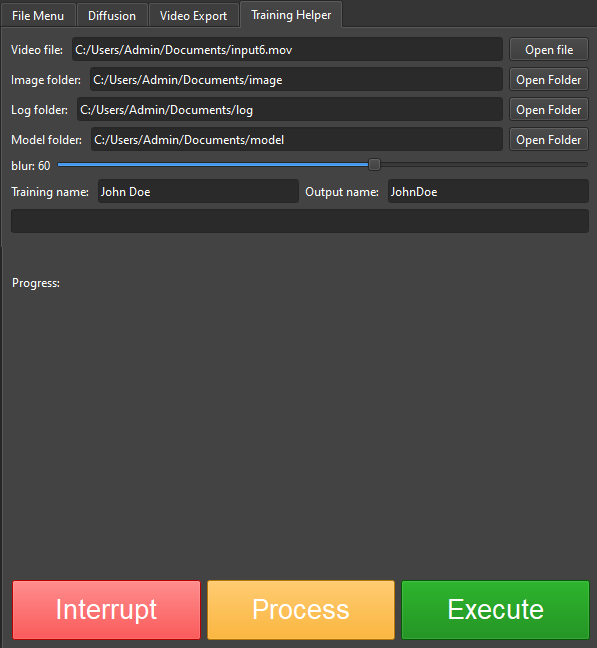
\includegraphics[scale=0.3, keepaspectratio]{img/project_img/training-help.png}
	\caption{The training helper window.}
	\label{fig:training-helper}
\end{figure}


The training helper window (Fig. \ref{fig:training-helper}) offers a companion for the 
LoRA training webUI (Section \ref{fig:lora-webui}). 
The window comprises \textbf{one file input} for the dataset video and \textbf{three directory inputs} 
for the directories needed for the LoRA training. 
The ``\textbf{blur}'' slider represents the threshold for the blur detection algorithm. 
The ``\textbf{Training name}'' is the identifier inserted in the BLIP captions, 
while the ``\textbf{Output name}'' is the model's name, the same one used during diffusion. 
Finally, a progress bar with its label explicitly shows the overall progress.
The ``\textbf{Process}'' button creates the necessary directories and starts processing the 
input video, as described in Section \ref{fig:lora-webui}, while the ``\textbf{Execute}'' button generates the 
JSON configuration file needed for training.
Finally, as said before, the ``\textbf{Interrupt}'' button allows the user to interrupt the processing.



\subsection{Problems and Future Improvements}

\begin{figure}[t]
	\centering
	\begin{subfigure}[b]{0.5\textwidth}
		\centering
		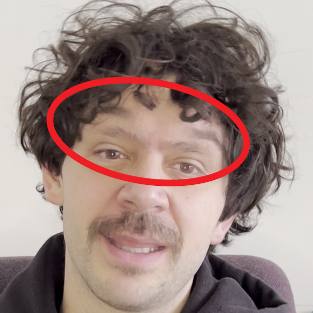
\includegraphics[scale=0.4]{img/project_img/error-eyebrows.png}
		\caption{Error on eyebrows.}\label{fig:error-eyebrows}
	\end{subfigure}%
	\hfill
	\begin{subfigure}[b]{0.5\textwidth}
		\centering
		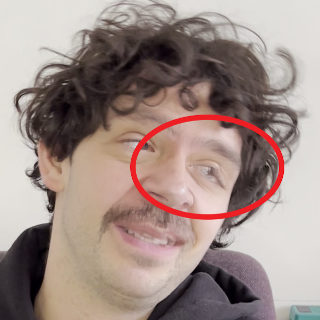
\includegraphics[scale=0.4]{img/project_img/error-eyes.png}
		\caption{Error on eyes.}\label{fig:error-eyes}
	\end{subfigure}
	\caption{Examples of errors.}\label{fig:errors}
\end{figure}
Even though the software can give consistent results, these are far from perfect. 
In fact, during the development, the main focus was on achieving a \textbf{non-detectable Deepfake}. 
The \emph{frame-to-frame coherence} problem was resolved through ControlNet 
canny model used on cropped frames with a locked noise seed. 
Some examples of detectable problems can be seen in Fig \ref{fig:error-eyebrows} and Fig \ref{fig:error-eyes}, 
where the software creates distorted faces. 
These problems can be resolved in the future by implementing a better 
\emph{mask-creation algorithm} or even allowing the user to re-generate only broken frames.
We still need to find out what a new and continuously improving technology like 
Stable Diffusion could do in the following years so that the solution might be completely different. 
The final video is still a 12 FPS video, so implementing an \emph{ML-based frame interpolator} could achieve 
24 or even 60 FPS for more fluidity. 
The GUI presented was to test all the components organically. 
However, the software could effortlessly become a \textbf{mobile application}, 
doing heavy calculations on a server, opening the possibility to widespread use.



\section{Conclusion}\label{ch:conclusion}
In conclusion, this thesis has proposed a novel approach to Deepfake creation using Stable Diffusion, ControlNet, and LoRA. By combining these three techniques, we have shown that creating highly realistic and almost stable Deepfakes with complete control over their features and quality is possible. Furthermore, we have demonstrated how to fine-tune a Stable Diffusion model through LoRA,  allowing us to generate new faces not present in the original datasets. How ControlNet can help us achieve more frame-to-frame consistency during the diffusion process, and finally, how all these models can be implemented in a single standalone application to generate Deepfakes. Since MediaPipe supports multi-face detection, future versions of this software could expand the possibilities to a multi-face Deepfake solution. Given that this solution could be slow with the current pipeline, a possibility is to distribute the diffusion process on multiple machines. This strategy could also give the possibility to do all the calculations on remote servers allowing the software to become a lightweight client app on a mobile phone. The mobile application could also help the Deepfake technology to become easier to employ for a larger number of users due to the low need for processing power. In future software versions, there will be the possibility to manage ControlNet parameters and change the current ControlNet model, making the diffusion process easier to adjust to the user's needs.
The current software does not replicate the original audio to the output video. To solve this problem, we could copy the original audio to the final video or implement an ML-based solution to generate the audio with the target subject's voice. However, this last solution also creates the need to implement a training strategy for the audio component. Finally, the last improvement could be an ML-based frame interpolation strategy, resulting in a 24 FPS or even 60 FPS output video.

\bibliographystyle{elsarticle-num}  
\bibliography{biblio}




\end{document}



